\chapter{Droite dans le plan}\label{droite_plan}

\section{Rappel}

Commençons par rappeler la définition du plan et des notions associées :

\begin{definition}
Le \emph{plan}\index{plan} est l'ensemble des couples $(x;y)$ avec $x,y\in \R$. On peut ainsi le représenter comme une feuille infinie.

Pour s'y repérer, nous utiliserons deux axes gradués, perpendiculaires et se croisant sur le point $(0;0)$.

Le premier axe, horizontal, s'appelle l'\emph{abscisse}\index{abscisse} et le second, vertical, l'\emph{ordonnée}\index{ordonnée}. Le point $(0;0)$, quant à lui, s'appelle l'\emph{origine}\index{origine}.
\end{definition}

\begin{center}
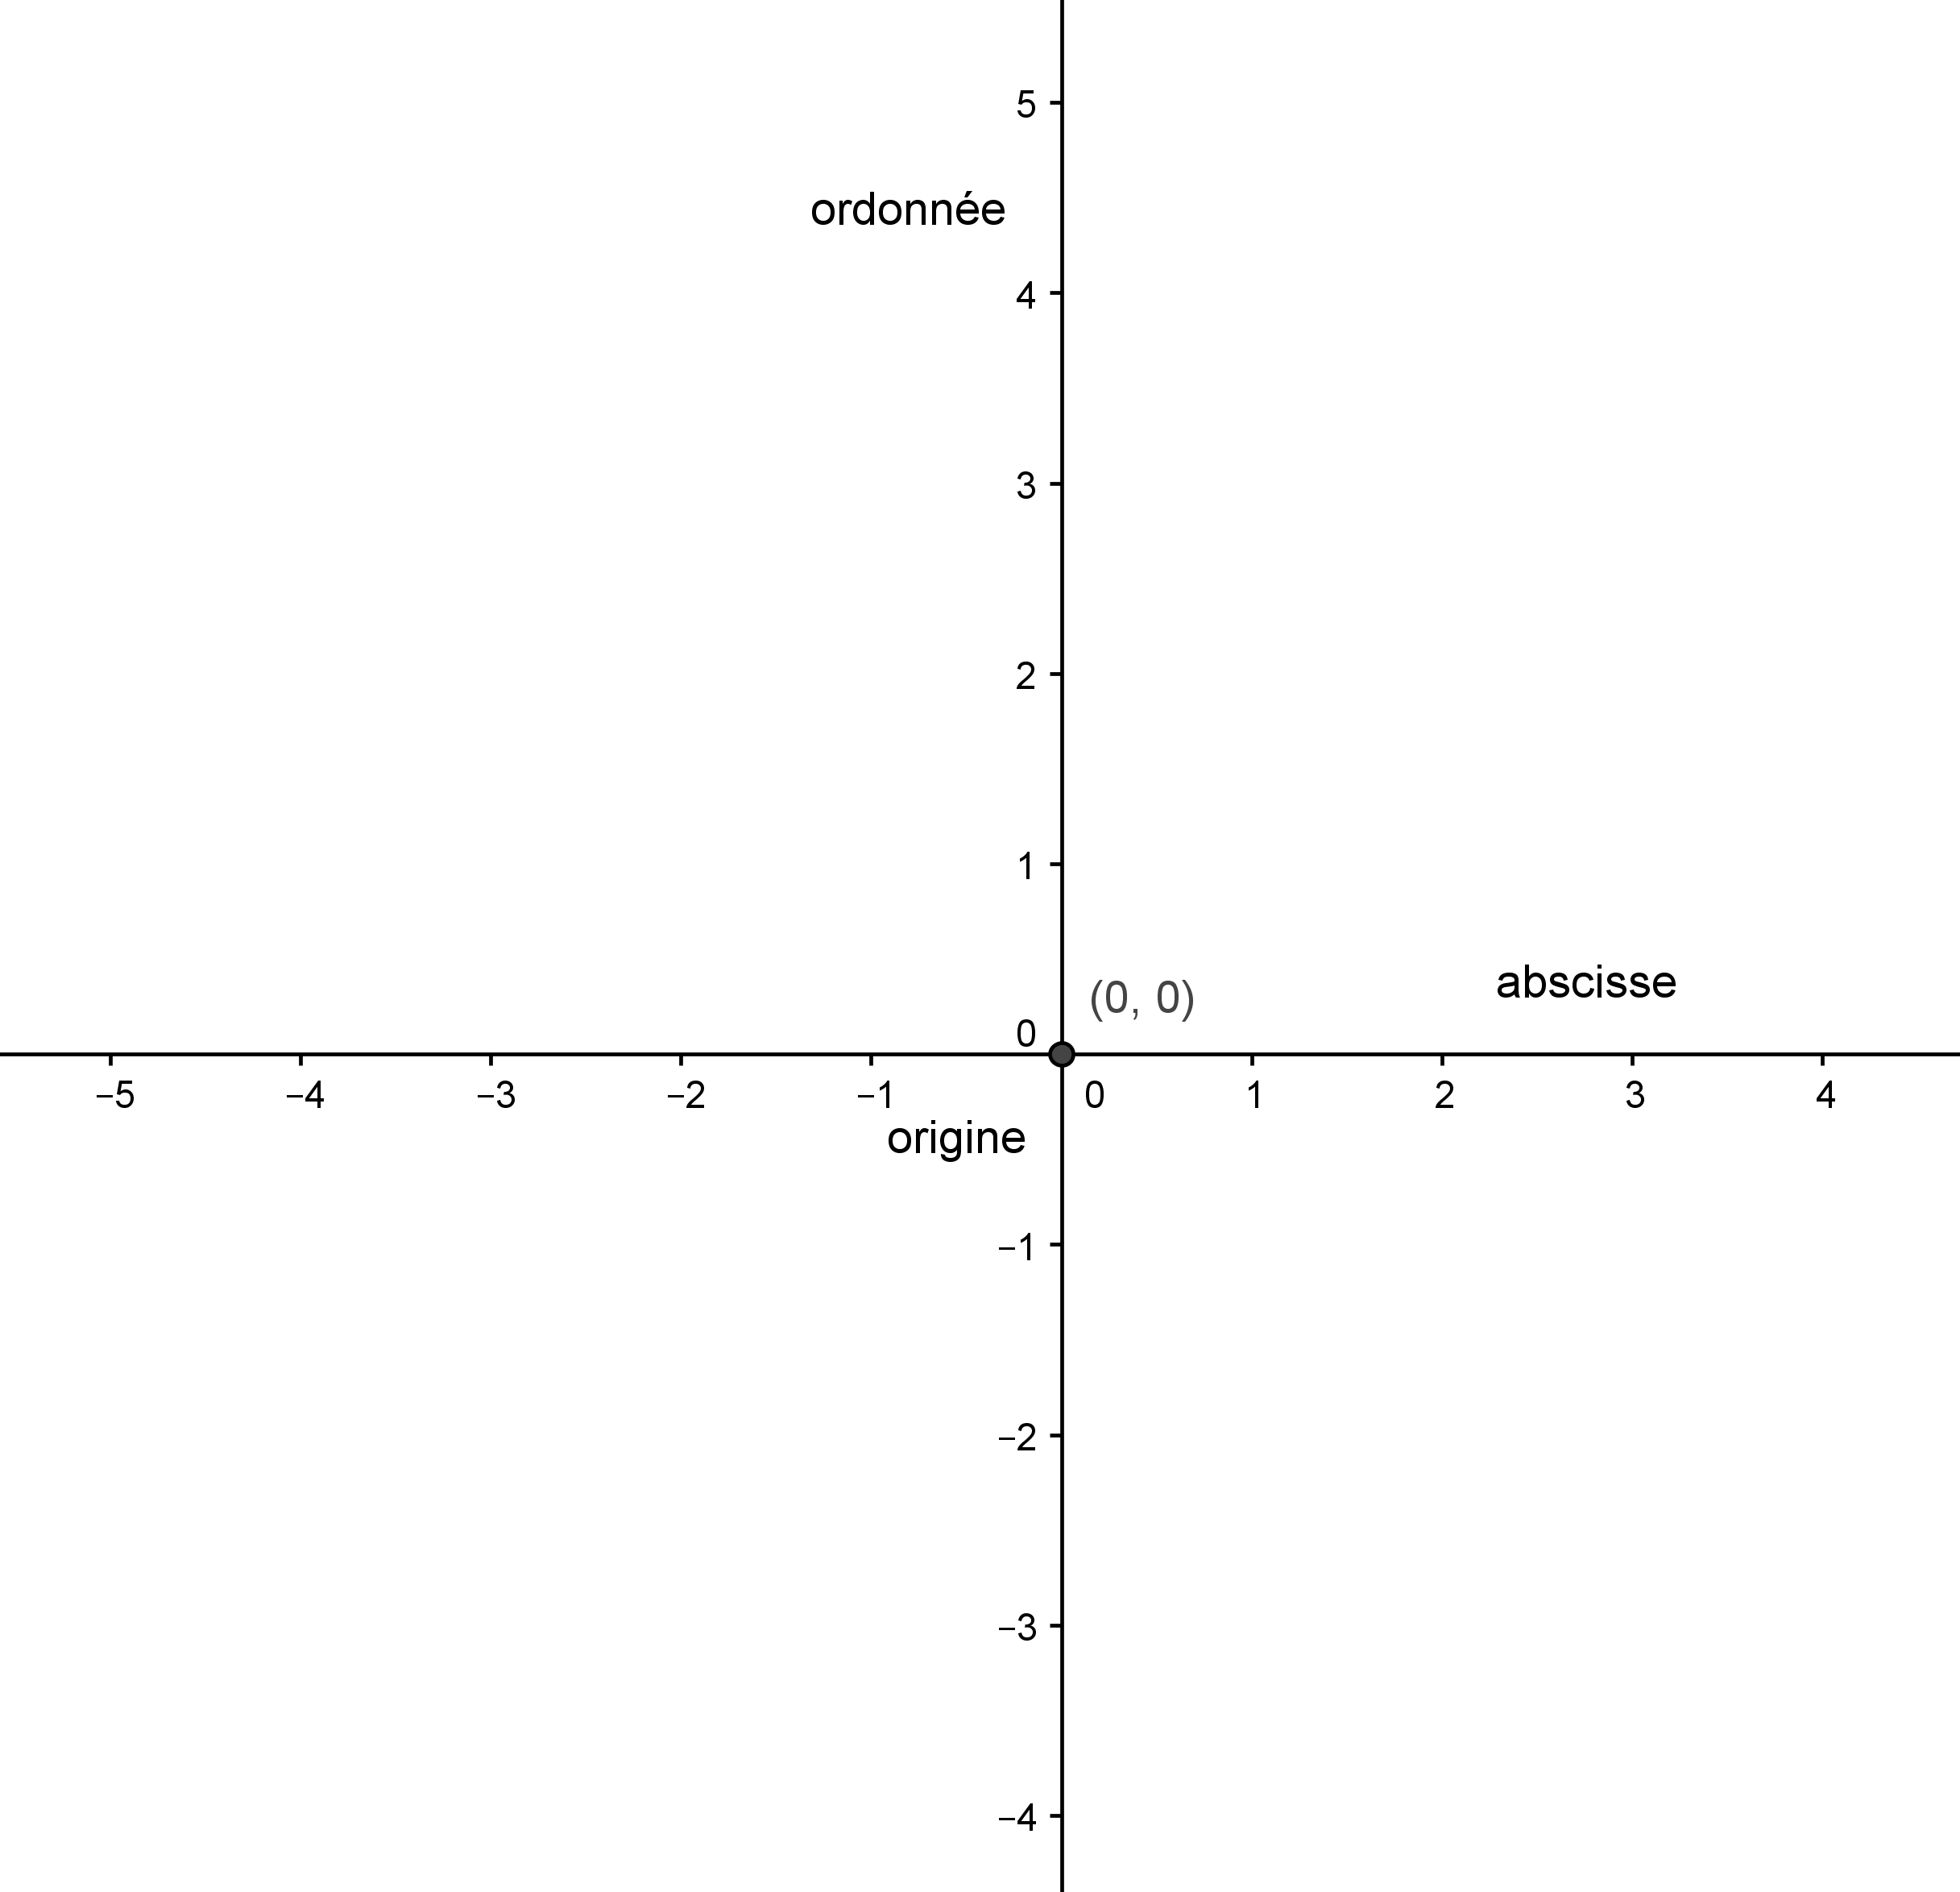
\includegraphics[width = 0.9 \textwidth]{droite/plan.png}
\end{center}

Sur le plan, tout point peut être représenté selon ses deux coordonnées $x$ et $y$ comme nous l'avons vu à la section~\ref{fct_representation}.

Aussi, de manière générale, nous parlerons du point
$$
P(x_P;y_P)
$$

Par exemple, pour le point $A(3;-2)$, on a $x_A = 3$ et $y_A = -2$. Cette notion est très importante et nous l'utiliserons dans tout ce chapitre !

\section{Droite}

Euclide\index{Euclide}, en $300$ avant J.-C., écrivait à propos de la droite :
\begin{quote}
\begin{enumerate}
\item Une ligne est une longueur sans largeur.\label{def_droite}
\item  Un segment de droite peut être tracé en joignant deux points quelconques.\label{elt_un}
\item Un segment de droite peut être prolongé indéfiniment en une ligne droite.\label{elt_deux}
\item Étant donné un segment de droite quelconque, un cercle peut être tracé en prenant ce segment comme rayon et l'une de ses extrémités comme centre.\label{elt_trois}
\item Tous les angles droits sont congruents.\label{elt_quatre}
\item Si deux lignes droites sont sécantes avec une troisième de telle façon que la somme des angles intérieurs d'un côté est inférieure à deux angles droits, alors ces deux lignes sont forcément sécantes de ce côté.\label{elt_cinq}
\end{enumerate}
\end{quote}
Pour nous, seule les éléments~(\ref{def_droite}), (\ref{elt_un}) et (\ref{elt_deux}) concernent la droite. Mais il est intéressant de voir que ces notions intéressaient les grecs déjà dans l'antiquité. C'est aussi dans l'histoire l'une des premières fois que la notion d'infini appara\^it.

Pour nous, nous définirons la notion de droite via la \emph{géométrie analytique} :

\begin{definition}
Une \emph{droite} est un ensemble de point vérifiant une équation à deux inconnues linéaire du type
$$\begin{array}{l}
ax+by=c, \mbox{ avec } a,b,c\in \R \mbox{ forme implicite}\\
y = mx + h, \mbox{ avec } m,h\in \R \mbox{ forme explicite}
\end{array}
$$
\end{definition}

Remarquons dans cette définition que la forme explicite ressemble fortement à une fonction affine (section~\ref{fct_affine}). Nous utiliserons des notions de fonction pour les droites par la suite.

On voit peu le lien entre cette définition et l'idée, toute simple, que l'on peut se faire d'une droite. Voyons cela de plus près avec un exemple :

\begin{exemple}
Soit la droite $d:2x+5y = 10$. Une première question serait : comment savoir si un point $P$ est sur la droite $d$. Prenons donc un point $P(3;2)$ au hasard. Pour savoir si $P$ est sur la droite, il convient d'appliquer l'équation de la droite au point :
$$
\begin{array}{rcl}
P &\in^?& d \ssi \\
d:2x_P + 5y_P &=^?& 10\ssi \\
2\cdot 3 + 5 \cdot 2 &=^?& 10 \ssi \\
6 + 10 &=^?& 10 \ssi \\
16 &=^?& 10
\end{array}
$$
Puisque manifestement $16\neq 10$, le point $P$ n'est pas sur la droite $d$.

Dès lors, comment trouver un point qui est sur la droite $d$ ? Puisque nous avons une seule équation et deux inconnues, nous pouvons sans problème fixer une coordonnée, c'est-à-dire attribuer une valeur au hasard à $x$ ou à $y$. Pour simplifier les calculs, commençons par poser $x=0$ :
$$
\begin{array}{lcl}
2 \cdot 0 + 5 y &=& 10 \ssi \\
5y  &=& 10 \ssi \\
y &=& 2.
\end{array}
$$
Ainsi puisque nous avons posé $x=0$ et que nous avons trouvé $y=2$, la droite $d$ passe par le point $A(0;2)$. C'est déjà un début, mais pour rejoindre le point de vue d'Euclide sur la droite, il nous faut un deuxième point. Naturellement regardons ce qui se passe si $y=0$ :
$$
\begin{array}{lcl}
2x + 5\cdot 0 &=& 10 \ssi \\
2x &=& 10 \ssi \\
x &=& 5.
\end{array}
$$
Ainsi puisque nous avons posé $y=0$ et que nous avons trouvé $x=5$, la droite $d$ passe par le point $B(5;0)$. Si on devait la dessiner, on trouverait :
\begin{center}
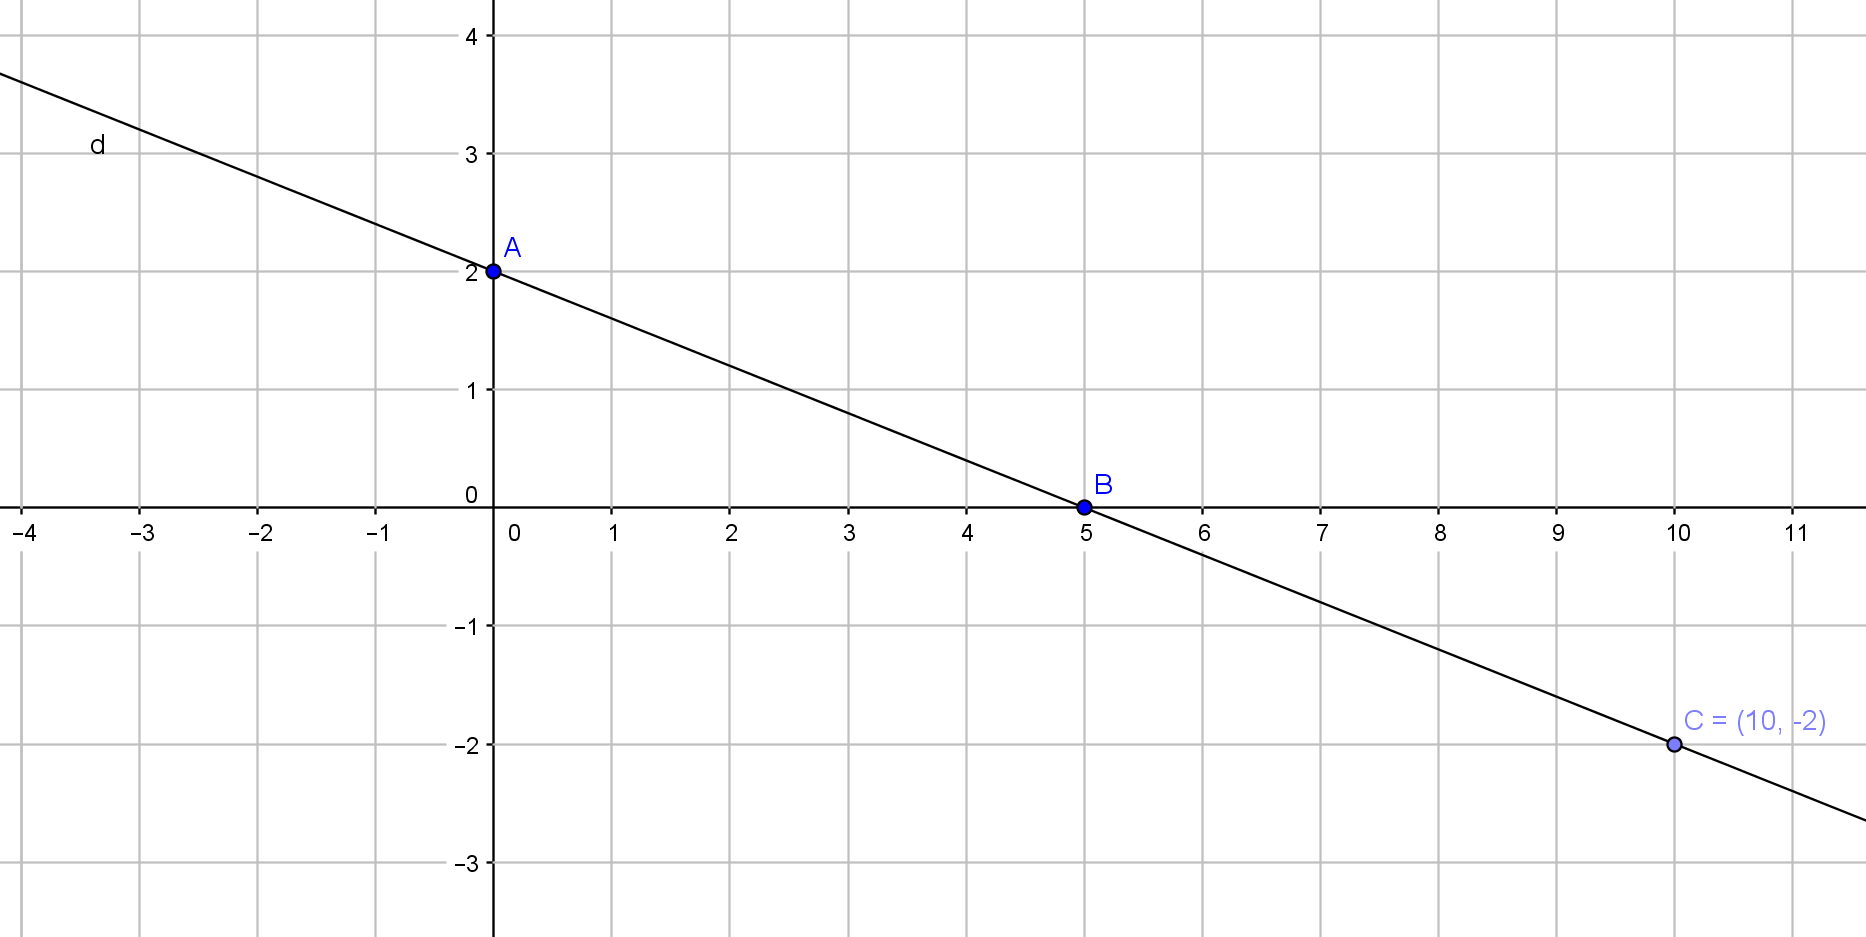
\includegraphics[width = 0.9\textwidth]{droite/droite_ex.png}
\end{center}
On remarque que la droite passe aussi par le point $C(10;-2)$, mais est-ce que ce point vérifie l'équation de la droite $d$ ?
$$
\begin{array}{rcl}
C &\in^?& d \ssi \\
d:2x_C + 5y_C &=^?& 10\ssi \\
2\cdot 10 + 5 \cdot (-2) &=^?& 10 \ssi \\
20 - 10 &=^?& 10 \ssi \\
10 &=^?& 10
\end{array}
$$
Puisque manifestement $10 = 10$, le point $C$ est sur la droite $d$. Or il en est de même pour les autres points de la droite et l'on voit ainsi comment les notions d'Euclide et de géométrie analytique se rejoignent.
\end{exemple}

Intéressons-nous maintenant à une notion déjà aperçue dans la section des fonctions affines : la pente.

\begin{definition}
La \emph{pente}\index{pente!d'une droite} entre deux points $A$ et $B$ du plan est donnée par 
$$
\mbox{pente } = \frac{\mbox{distance verticale entre }A\mbox{ et }B}{\mbox{distance horizontale entre }A\mbox{ et }B}
$$
\end{definition}

Comme on le voit sur le graphique suivant, la pente d'une droite est donnée par la formule
$$
\mbox{pente } = \frac{y_B-y_A}{x_B-x_A}
$$

\begin{center}
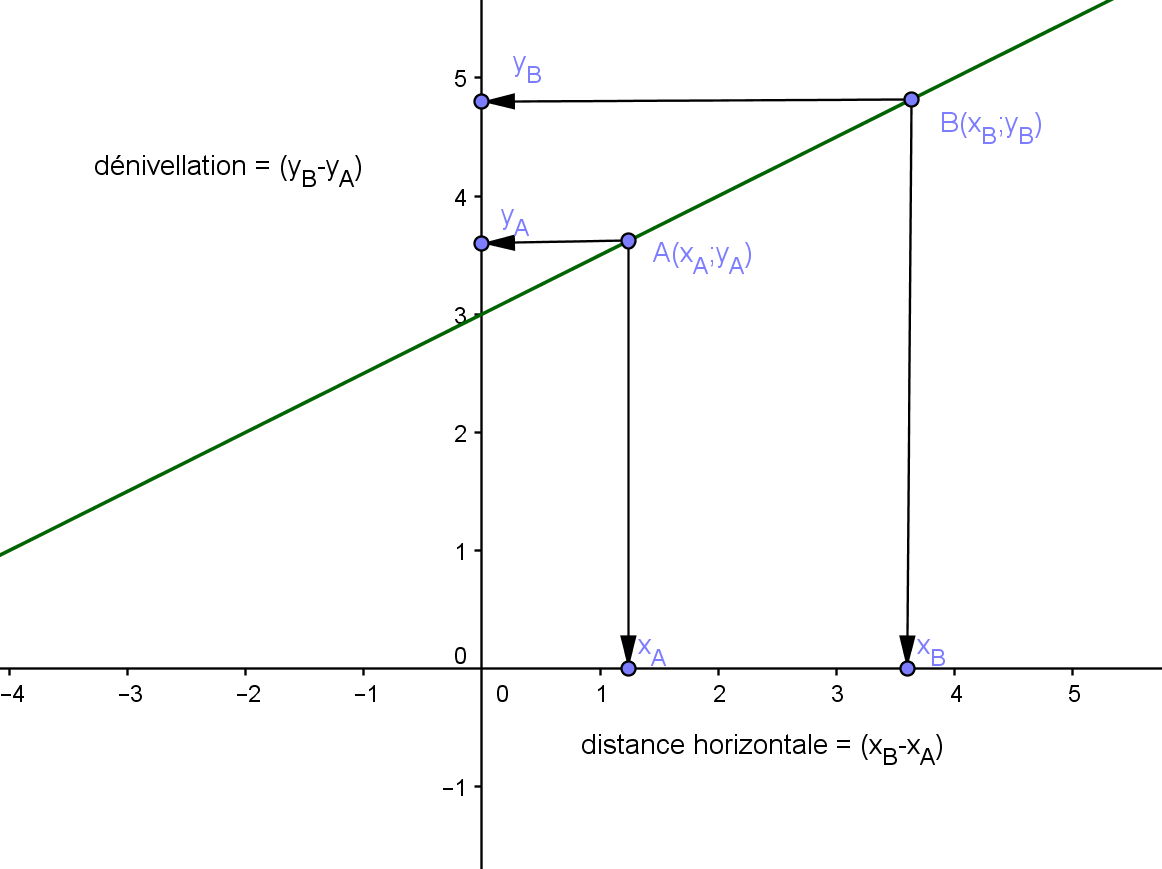
\includegraphics[width=0.9 \textwidth]{droite/droite_pente.png}
\end{center}

\begin{theoreme}
La pente d'une droite est donnée par $m$ dans sa forme explicite.
\end{theoreme}

\begin{proof}
Soit une droite $d:y = mx+h$ et soient $A$ et $B$ deux points sur la droite. Ainsi
$$
\left\{
\begin{array}{lcl}
y_A &=& mx_A + h\\
y_B &=& mx_B + h
\end{array}
\right.
$$
Si l'on soustrait ces deux équations et que l'on isole $m$ on obtient :
$$
\begin{array}{lcl}
y_B-y_A &=& (mx_B + h)-(mx_A + h)\ssi \\
y_B-y_A &=& mx_B + h-mx_A - h\ssi \\
y_B-y_A &=& mx_B-mx_A \ssi \\
(y_B-y_A) &=& m(x_B-x_A)\ssi \\
\frac{(y_B-y_A)}{(x_B-x_A)} &=& m\ssi \\
\end{array}
$$
ce qui démontre que $m$ est la pente de la droite $d$.
\end{proof}

\subsection{Parallèle}

En géométrie euclidienne, on dit que deux droites sont parallèles si et seulement si elles n'ont aucune intersection. Avec le postulat~(\ref{elt_cinq}) que l'on trouve au début de ce chapitre on peut conclure que par un point passe une seule parallèle à une autre droite. Cette notion parait tellement triviale que durant longtemps les mathématiciens ont essayé de la démontrer. Euler~\index{Euler}, un mathématicien suisse du 18e siècle a proposé d'autres modèles de géométrie, typiquement la géométrie sur une sphère, où cette propriété n'est pas vérifiée (c'est-à-dire qu'on peut faire passer plusieurs parallèles par le même point).

\begin{proposition}
En géométrie euclidienne, deux droites sont parallèles si et seulement si elles ont la même pente.
\end{proposition}

Cette proposition ne sera pas démontrée, une compréhension graphique suffit.

\subsection{Perpendiculaires}

La notion de perpendiculaire est, au sein de notre progression, difficile à définir. En effet, nous n'avons pas défini la notion d'angle. Aussi nous considérerons la notion de perpendicularité comme intuitive, par exemple s'il est possible de dessiner un carré ayant chacune des deux droites sécantes comme diagonales.

\begin{proposition}
Soient $d_1$ et $d_2$ deux droites ayant respectivement les pentes $m_1$ et $m_2$. Alors les deux droites sont perpendiculaires si et seulement si
$$
m_1 = \frac{-1}{m_2}.
$$
\end{proposition}

\begin{proof}
Voyons cette proposition par voie graphique et uniquement dans un sens :
\begin{center}
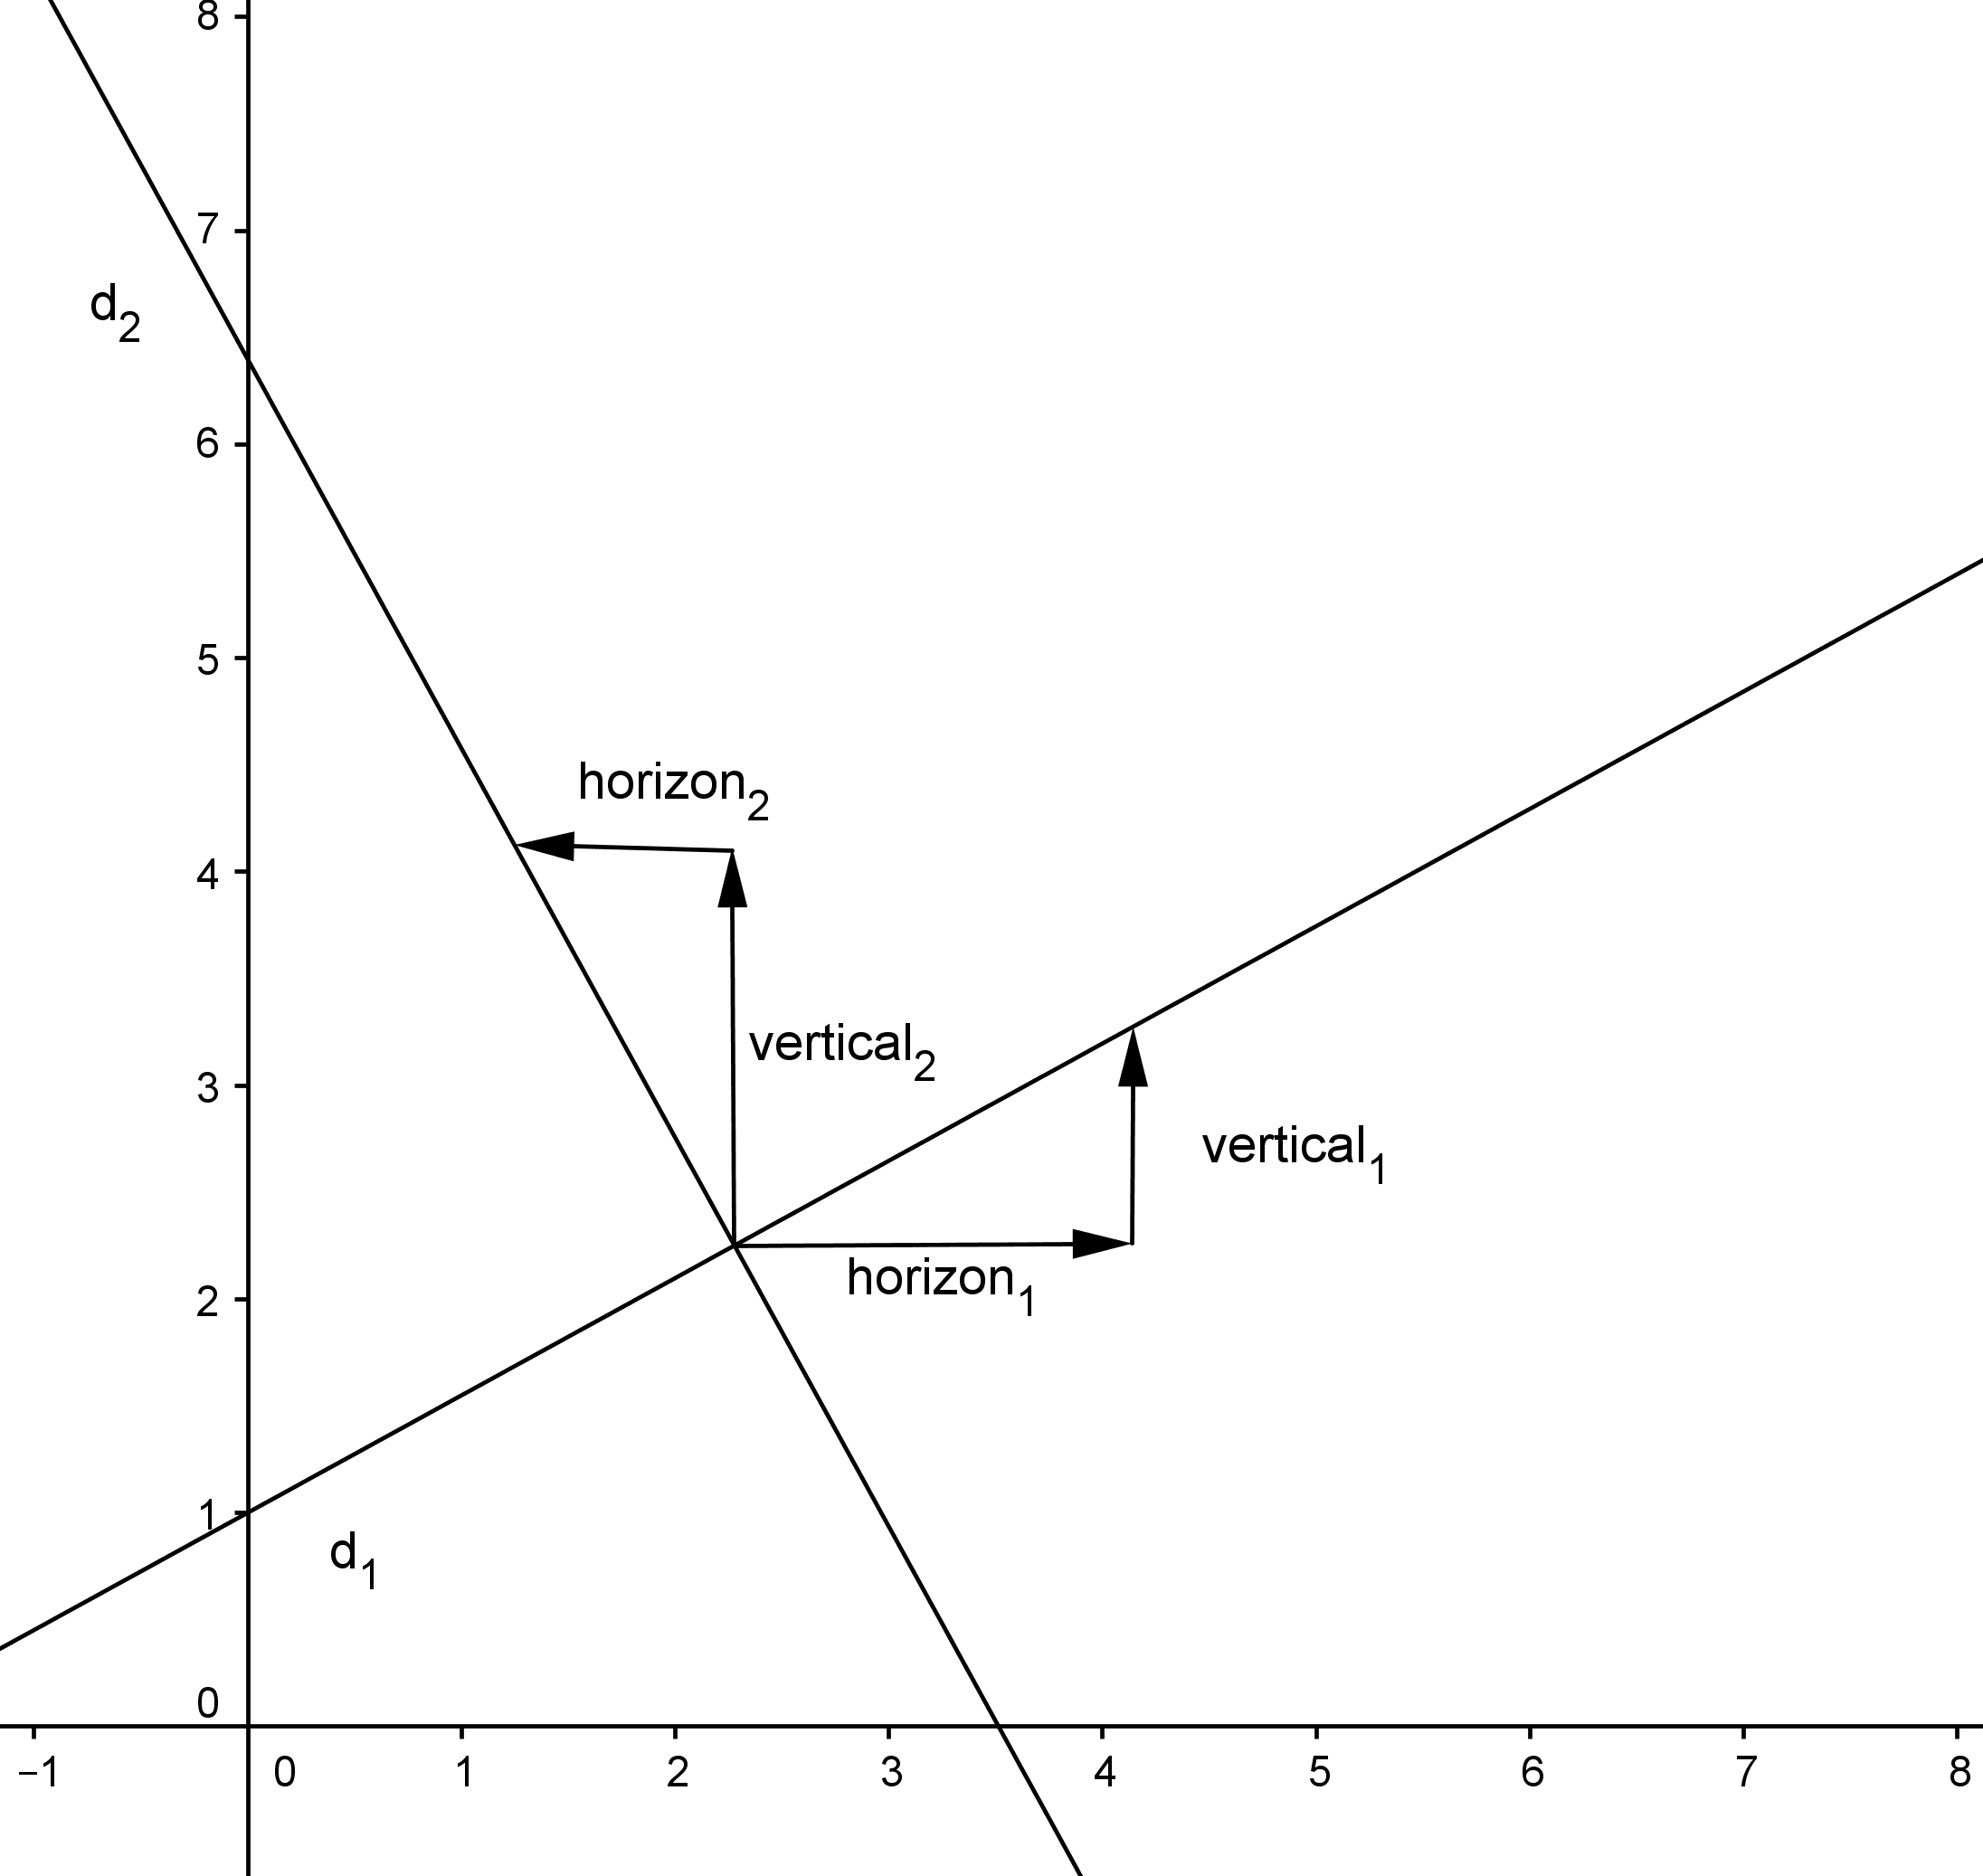
\includegraphics[width=0.9\textwidth]{droite/perpendiculaire.png}
\end{center}
On remarque que la verticale de $d_2$ est égale à l'horizontale de $d_1$ et que l'horizontale de $d_2$ est le contraire de la verticale de $d_1$.
Ainsi 
$$
\begin{array}{lcl}
m_1 &=& \frac{\mbox{vertical}_1}{\mbox{horizontal}_1}\\
&=& \frac{-\mbox{horizontal}_2}{\mbox{vertical}_2}\\
&=& \frac{-1}{\frac{\mbox{vertical}_2}{\mbox{horizontal}_2}}\\
&=& \frac{-1}{m_2}.
\end{array}
$$
Une partie de la proposition est ainsi démontrée. Il nous faudrait encore voir que si deux droites respectent l'égalité liée aux pentes, alors elles sont perpendiculaires, mais comme notre définition de perpendiculaire est très intuitive, elle complique la démonstration.
\end{proof}

\section{Exercices}

\begin{exercice}
\'Etudier toutes les caractéristiques des droites suivantes (formes implicites).
	Tracer au maximum deux droites sur un même système d'axes, unité des axes : un carré.
\begin{multicols}{2}
\begin{enumerate}
\item $x+y=5$
\item $x-y=-3$
\item $2x+y=6$
\item $x-3y=12$
\item $3x+2y=6$
\item $-2x+3y=6$
\item $-3x-5y=30$
\item $5x+2y=-20$
\item $7x-2y=-28$
\item $3x-4y=9$
\item $-4x+5y=-15$
\item $2x+3y=5$
\item $y=-4$
\item $5y=35$
\item $x=6$
\item $-3x=12$
\end{enumerate}
\end{multicols}
\end{exercice}

\begin{exercice}
Calculer les équations des droites suivantes, connaissant la pente p et les coordonnées d'un point A de la droite. Donner les formes explicites et implicites des équations de droites.
\begin{multicols}{2}
\begin{enumerate}
\item $p=1\text{     }A(1;2)$
\item $p=3\text{     }A(-1;3)$
\item $p=-4\text{     }A(5;-5)$
\item $p=-7\text{     }A(-4;-3)$
\item $p=\frac{1}{2}\text{     }A(4;12)$
\item $p=\frac{4}{5}\text{     }A(-9;5)$
\item $p=-\frac{8}{3}\text{     }A(0;3)$
\item $p=-\frac{11}{13}\text{     }A(-5;0)$
\item $p=\frac{127}{19}\text{     }A(0;0)$
\item $p=\frac{34}{11}\text{     }A(-7;15)$
\item $p=0\text{     }A(4;5)$
\item $p=\infty \text{     }A(4;5)$
\end{enumerate}
\end{multicols}
\end{exercice}

\begin{exercice}
Calculer les équations des droites suivantes, connaissant les coordonnées de deux points A et B de la droite. Donner les formes explicites et implicites des équations de droites.
\begin{multicols}{2}
\begin{enumerate}
\item $$ \left| \begin{array}{l}
 A(2;3) \\ 
B\left( 1;5 \right) \\ 
\end{array} \right.$$
\item $$\left| \begin{array}{l}
 A(12;7) \\ 
B\left( -2;5 \right) \\ 
\end{array} \right.$$
\item $$\left| \begin{array}{l}
 A(-11;-7) \\ 
B\left( 1;1 \right) \\ 
\end{array} \right.$$
\item $$\left| \begin{array}{l}
 A(5;7) \\ 
B\left( -3;-9 \right) \\ 
\end{array} \right.$$
\item $$\left| \begin{array}{l}
 A(-6;4) \\ 
B\left( 7;-2 \right) \\ 
\end{array} \right.$$
\item $$\left| \begin{array}{l}
 A(10;-12) \\ 
B\left( -4;5 \right) \\ 
\end{array} \right.$$
\item $$\left| \begin{array}{l}
 A(3,5;5,5) \\ 
B\left( 2,5;7,5 \right) \\ 
\end{array} \right.$$
\item $$\left| \begin{array}{l}
 A(75;-37) \\ 
B\left( -1;8 \right) 
 \end{array} \right.$$
\item $$\left| \begin{array}{l}
 A(5;5) \\ 
B\left( 12;12 \right) \\ 
\end{array} \right.$$
\item $$\left| \begin{array}{l}
 A(2;-6) \\ 
B\left( 6;-18 \right) \\ 
\end{array} \right.$$
\item $$\left| \begin{array}{l}
 A(3;7) \\ 
B\left( 15;7 \right) \\ 
\end{array} \right.$$
\item $$\left| \begin{array}{l}
 A(-2;-3) \\ 
B\left( -2;6 \right) \\ 
\end{array} \right.$$
\end{enumerate}
\end{multicols}
\end{exercice}

\begin{exercice}
Calculer les coordonnées du point M, milieu du segment AB.
\begin{multicols}{2}
\begin{enumerate}
\item $$\left| \begin{array}{l}
 A\left( 6;8 \right) \\ 
B\left( 2;12 \right) \\ 
\end{array} \right.$$
\item $$\left| \begin{array}{l}
 A\left( -4;16 \right) \\ 
B\left( 6;-10 \right) \\ 
\end{array} \right.$$
\item $$\left| \begin{array}{l}
 A\left( 5;11 \right) \\ 
B\left( 3;-9 \right) \\ 
\end{array} \right.$$
\item $$\left| \begin{array}{l}
 A\left( -18;77 \right) \\ 
B\left( 25;34 \right) \\ 
\end{array} \right.$$
\item $$\left| \begin{array}{l}
 A\left( \frac{13}{2};-\frac{3}{4} \right) \\ 
B\left( -\frac{7}{3};\frac{3}{5} \right) \\ 
\end{array} \right.$$
\item $$\left| \begin{array}{l}
 A\left( 0;0 \right) \\ 
B\left( -16;24 \right) \\ 
\end{array} \right.$$
\end{enumerate}
\end{multicols}
\end{exercice}

\begin{exercice}
Calculer la longueur du segment AB.
\begin{multicols}{3}
\begin{enumerate}
\item $$\left| \begin{array}{l}
 A\left( 2;10 \right) \\ 
B\left( 5;12 \right) \\ 
\end{array} \right.$$
\item $$\left| \begin{array}{l}
 A\left( -8;5 \right) \\ 
B\left( 6;-2 \right) \\ 
\end{array} \right.$$
\item $$\left| \begin{array}{l}
 A\left( 0;0 \right) \\ 
B\left( -5;0 \right) \\ 
\end{array} \right.$$
\end{enumerate}
\end{multicols}
\end{exercice}

\begin{exercice}
Calculer l'équation de la droite passant par le point A et parallèle à la droite d.
\begin{multicols}{3}
\begin{enumerate}
\item $$\left| \begin{array}{l}
 A\left( 5;9 \right) \\ 
d:y=3x-5 \\ 
\end{array} \right.$$
\item $$\left| \begin{array}{l}
 A\left( -3;4 \right) \\ 
d:y=-\frac{5x}{2}+1 \\ 
\end{array} \right.$$
\item $$\left| \begin{array}{l}
 A\left( -7;-3 \right) \\ 
d:3x+7y=2 \\ 
\end{array} \right.$$
\end{enumerate}
\end{multicols}
\end{exercice}

\begin{exercice}
Calculer l'équation de la droite passant par le point A et perpendiculaire à la droite d.
\begin{multicols}{3}
\begin{enumerate}
\item $$\left| \begin{array}{l}
 A\left( 3;-2 \right) \\ 
d:y=2x-5 \\ 
\end{array} \right.$$
\item $$\left| \begin{array}{l}
 A\left( -6;0 \right) \\ 
d:y=\frac{3x}{7} \\ 
\end{array} \right.$$
\item $$\left| \begin{array}{l}
 A\left( -3;8 \right) \\ 
d:5x+2y=2 \\ 
\end{array} \right.$$
\end{enumerate}
\end{multicols}
\end{exercice}

\section{Corrigés}

\begin{solution}

\end{solution}

\begin{landscape}

\begin{solution}
Calculer les équations des droites suivantes, connaissant la pente p et les coordonnées d'un point A de la droite. Donner les formes explicites et implicites des équations de droites.
$$
\begin{array}{|l|l|l|l|l|l|}
\hline
1.          & 2.           & 3.            & 4.            & 5.                   & 6.                                \\ \hline
p = 1       & p = 3        & p =-4       & p =-7       & p=\frac{1}{2}     & p=\frac{4}{5}                  \\ \hline
A(1 ;2)     & A(- 1 ;3)    & A(5 ;-5)    & A(- 4 ;- 3)   & A(4 ;12)             & A(- 9 ;5)                         \\ \hline
y = x+b     & y = 3x + b   & y =-4x + b  & y =-7 x + b & y=\frac{1}{2}x+b  & y=\frac{4}{5}x+b               \\ \hline
2 = 1 + b   & 3 =-3 + b  & -5 =-20 + b &-3 = 28 + b  & 12 = 2 + b           & 5=-\frac{36}{5}+b              \\ \hline
b = 1       & b = 6        & b = 15        & b = -31       & b = 10               & b=\frac{61}{5}                 \\ \hline
y = x + 1   & y = 3x + 6   & y =-4x + 15 & y = -7 x-31 & y=\frac{1}{2}x+10 & y=\frac{4}{5}x+\frac{61}{5} \\ \hline
x-y =-1 & 3x-y =-6 & 4x + y = 15   & 7x + y =-31 & x-2y =-20        & 4x-5y =-61                    \\ \hline
\end{array}
$$

$$
\begin{array}{|l|l|l|l|l|l|}
\hline
7.                   & 8.                                    & 9.                     & 10.                                   & 11.         & 12.                                                                            \\ \hline
p=-\frac{8}{3}    & p=-\frac{11}{13}                   & p=\frac{127}{19}    & p=\frac{34}{11}                    & p=0         & p=infty                                                                        \\ \hline
A(0 :3)              & A(- 5 ;0)                             & A(0 ;0)                & A(- 7 ;15)                            & A(4 ;5)     & A(4 ;5)                                                                        \\ \hline
y=-\frac{8}{3}x+b & y=-\frac{11}{13}x+b                & y=\frac{127}{19}x+b & y=\frac{34}{11}x+b                 & y=0x+b      & \begin{array}[c]{@{}l@{}}Droite verticale d’équation \\   x = 4\end{array} \\ \hline
3 = b                & 0=\frac{55}{13}+b                  &                        & 15=-\frac{238}{11}+b               & 5=0cdot 4+b &                                                                                \\ \hline
b = 3                & b=-\frac{55}{13}                   & b = 0                  & b=\frac{403}{11}                   & b=5         &                                                                                \\ \hline
y=-\frac{8}{3}x+3 & y=-\frac{11}{13}x-\frac{55}{13} & y=\frac{127}{19}x   & y=\frac{34}{11}x+\frac{403}{11} & y=5         &                                                                                \\ \hline
8x+3y=9              & 11x + 13y =-55                      & 127x-19y = 0         & 34x -11y = -403                       &             &                                                                                \\ \hline
\end{array}
$$
\end{solution}

\end{landscape}

\begin{solution}
Calculer les équations des droites suivantes, connaissant les coordonnées de deux points A et B de la droite. Donner les formes explicites et implicites des équations de droites.
$$
\begin{array}{|l|l|l|l|l|l|}
\hline
1.                                                          & 2.                                                             & 3.                                                               & 4.                                                              & 5.                                                              & 6.                                                                \\ \hline
\begin{array}[c]{@{}l@{}}A(2 ;3)\\   B(1 ;5)\end{array} & \begin{array}[c]{@{}l@{}}A(12 ;7)\\   B(- 2 ;5)\end{array} & \begin{array}[c]{@{}l@{}}A(- 11 ;- 7)\\   B(1 ;1)\end{array} & \begin{array}[c]{@{}l@{}}A(5 ;7)\\   B(- 3 ;- 9)\end{array} & \begin{array}[c]{@{}l@{}}A(- 6 ;4)\\   B(7 ;- 2)\end{array} & \begin{array}[c]{@{}l@{}}A(10 ;- 12)\\   B(- 4 ;5)\end{array} \\ \hline
a=\frac{5-3}{1-2}                                        & a=\frac{5-7}{-2-12}                                         & a=\frac{1+7}{1+11}                                            & a=\frac{-9-7}{-3-5}                                          & a=\frac{-2-4}{7+6}                                           & a=\frac{5+12}{-4-10}                                           \\ \hline
a =-2                                                     & a=\frac{1}{7}                                               & a=\frac{2}{3}                                                 & a = 2                                                           & a=-\frac{6}{13}                                              & a=-\frac{17}{14}                                               \\ \hline
y=-2x+b                                                     & y=\frac{1}{7}x+b                                            & y=\frac{2}{3}x+b                                              & y=2x+b                                                          & y=-\frac{6}{13}x+b                                           & y=-\frac{17}{14}x+b                                            \\ \hline
3=-4+b                                                      & 5=-\frac{2}{7}+b                                            & 1=\frac{2}{3}+b                                               & 7=10+b                                                          & -2=-\frac{42}{13}+b                                          & 5=\frac{34}{7}+b                                               \\ \hline
b = 7                                                       & b=\frac{37}{7}                                              & b=\frac{1}{3}                                                 & b=-3                                                            & b=\frac{16}{13}                                              & b=\frac{1}{7}                                                  \\ \hline
y=-2x+7                                                     & y=\frac{1}{7}x+\frac{37}{7}                              & y=\frac{2}{3}x+\frac{1}{3}                                 & y=2x-3                                                          & y=-\frac{6}{13}x+\frac{16}{13}                            & y=-\frac{17}{14}x+\frac{1}{7}                               \\ \hline
2x + y = 7                                                  & x-7y =-37                                                  & 2x-3y =-1                                                    & 2x-y = 3                                                      & 6x + 13y = 16                                                   & 17x + 14y = 2                                                     \\ \hline
\end{array}
$$

$$
\begin{array}{|l|l|l|l|l|l|}
\hline
7.                                                                  & 8.                                                                & 9.                                                            & 10.                                                              & 11.                                                          & 12.                                                               \\ \hline
\begin{array}[c]{@{}l@{}}A(3.5 ;5.5)\\   B(2.5 ;7.5)\end{array} & \begin{array}[c]{@{}l@{}}A(75 ;- 37)\\   B(- 1 ;8)\end{array} & \begin{array}[c]{@{}l@{}}A(5 ;5)\\   B(12 ;12)\end{array} & \begin{array}[c]{@{}l@{}}A(2 ;- 6)\\   B(6 ;- 18)\end{array} & \begin{array}[c]{@{}l@{}}A(3 ;7)\\   B(15 ;7)\end{array} & \begin{array}[c]{@{}l@{}}A(- 2 ;- 3)\\   B(- 2 ;6)\end{array} \\ \hline
a=\frac{7.5-5.5}{2.5-3.5}                                        & a=\frac{8+37}{-1-75}                                           & a=\frac{12-5}{12-5}                                        & a=\frac{-18+6}{6-2}                                           & a=0                                                          & a=\frac{9}{0}=infty                                            \\ \hline
a =-2                                                             & a=-\frac{45}{76}                                               & a = 1                                                         & a =-3                                                          & y = b                                                        & Droite verticale                                                  \\ \hline
y=-2x+b                                                             & y=-\frac{45}{76}x+b                                            & y=x+b                                                         & y=-3x+b                                                          & b = 7                                                        & d’éq. x =-2                                                     \\ \hline
5.5=-7+b                                                            & 8=\frac{45}{76}+b                                              & 5=5+b                                                         & -6=-6+b                                                          & y = 7                                                        &                                                                   \\ \hline
b=\frac{25}{2}                                                   & b=\frac{563}{76}                                               & b=0                                                           & b=0                                                              &                                                              &                                                                   \\ \hline
y=-2x+\frac{25}{2}                                               & y=-\frac{45}{76}x+\frac{563}{76}                            & y=x                                                           & y=-3x                                                            &                                                              &                                                                   \\ \hline
4x+2y=25                                                            & 45x+76y=563                                                       & x-y=0                                                         & 3x+y=0                                                           &                                                              &                                                                   \\ \hline
\end{array}
$$
\end{solution}

\begin{solution}
Calculer les coordonnées du point M, milieu du segment AB :
$$
\begin{array}{|l|l|l|l|l|l|}
\hline
1.                                                           & 2.                                                               & 3.                                                            & 4.                                                               & 5.                                                                                                                                                                        & 6.                                                             \\ \hline
\begin{array}[c]{@{}l@{}}A(6 ;8)\\   B(2 ;12)\end{array} & \begin{array}[c]{@{}l@{}}A(- 4 ;16)\\   B(6;- 10)\end{array} & \begin{array}[c]{@{}l@{}}A(5 ;11)\\   B(3;- 9)\end{array} & \begin{array}[c]{@{}l@{}}A(- 18 ;77)\\   B(25;34)\end{array} & \begin{array}[c]{@{}l@{}}       A(\frac{13}{2};-\frac{3}{4})\\    \\      B(-\frac{7}{3};\frac{3}{5})\\    \\   \end{array} & \begin{array}[c]{@{}l@{}}A(0 ;0)\\   B(- 16;24)\end{array} \\ \hline
(4 ;10)                                                      & (1;3)                                                            & (4;1)                                                         & (\frac{7}{2};\frac{111}{2})                                & (\frac{25}{12};-\frac{3}{40})                                                                                                                                       & (- 8;12)                                                       \\ \hline
\end{array}
$$
\end{solution}

\begin{solution}
Calculer la longueur  du segment AB :
$$
\begin{array}{|l|l|l|}
\hline
\begin{array}[c]{@{}l@{}}A(2 ;10)\\   B(5 ;12)\end{array}                                                   & \begin{array}[c]{@{}l@{}}A(- 8 ;5)\\   B(6 ;- 2)\end{array}                                                  & \begin{array}[c]{@{}l@{}}A(0 ;0)\\   B(- 5 ;0)\end{array}                                                   \\ \hline
{{\overline{AB}}\textasciicircum{}{2}}={{3}\textasciicircum{}{2}}+{{2}\textasciicircum{}{2}} & {{\overline{AB}}\textasciicircum{}{2}}={{14}\textasciicircum{}{2}}+{{7}\textasciicircum{}{2}} & {{\overline{AB}}\textasciicircum{}{2}}={{5}\textasciicircum{}{2}}+{{0}\textasciicircum{}{2}} \\ \hline
\overline{AB}=\sqrt{9+4}                                                                                      & \overline{AB}=\sqrt{196+49}                                                                                    & \overline{AB}=\sqrt{25}                                                                                       \\ \hline
\overline{AB}=\sqrt{13}                                                                                       & \overline{AB}=7\sqrt{5}                                                                                        & \overline{AB}=5                                                                                                \\ \hline
\end{array}
$$
\end{solution}

\begin{solution}
Calculer l'équation de la droite passant par le point A et parallèle à la droite d :
$$
\begin{array}{|l|l|l|}
\hline
\begin{array}[c]{@{}l@{}}      A(5;9)  \\     d:y=3x-5  \\   \end{array} & \begin{array}[c]{@{}l@{}}       A(-3;4)  \\   d:y=-\frac{5}{2}x+1  \\   \end{array} & \begin{array}[c]{@{}l@{}}     \\   A(-7;-3)  \\    \\   d:3x+7y=2  \\   \end{array} \\ \hline
Parallèle :                                                                                                  & Parallèle :                                                                                                                 & Parallèle :                                                                                                             \\ \hline
y=3x+b                                                                                                       & y=-\frac{5}{2}x+b                                                                                                        & y=-\frac{3}{7}x+b                                                                                                    \\ \hline
9=15+b                                                                                                       & 4=\frac{15}{2}+b                                                                                                         & -3=3+b                                                                                                                  \\ \hline
b=-6                                                                                                         & b=-\frac{7}{2}                                                                                                           & b=-6                                                                                                                    \\ \hline
y=3x-6                                                                                                       & y=-\frac{5}{2}x-\frac{7}{2}                                                                                           & y=-\frac{3}{7}x-6                                                                                                    \\ \hline
3x-y=6                                                                                                    & 5x+2y=-7                                                                                                                  & 3x+7y=-42                                                                                                             \\ \hline
\end{array}
$$
\end{solution}

\begin{solution}
Calculer l'équation de la droite passant par le point A et perpendiculaire à la droite d :
$$
\begin{array}{lll}
\begin{array}[c]{@{}l@{}}  A(3;-2)  \\     d:y=2x-5  \\   \end{array} & \begin{array}[c]{@{}l@{}}  A(-6;0)  \\     d:y=\frac{3}{7}x  \\   \end{array} & \begin{array}[c]{@{}l@{}}    A(-3;8)  \\       d:5x+2y=2  \\   \end{array} \\
Perpendiculaire :                                                                                             & Perpendiculaire :                                                                                                        & Perpendiculaire :                                                                                                      \\
y=-\frac{1}{2}x+b                                                                                          & y=-\frac{7}{3}x+b                                                                                                     & y=\frac{2}{5}x+b                                                                                                    \\
-2=-\frac{3}{2}+b                                                                                          & 0=\frac{42}{3}+b                                                                                                      & 8=-\frac{6}{5}+b                                                                                                    \\
b=-\frac{1}{2}                                                                                             & b=-\frac{42}{3}                                                                                                       & b=\frac{46}{5}                                                                                                      \\
y=-\frac{1}{2}x-\frac{1}{2}                                                                             & y=-\frac{7}{3}x-\frac{42}{3}                                                                                       & y=\frac{2}{5}x+\frac{46}{5}                                                                                      \\
x+2y=-1                                                                                                     & 7x+3y=-42
 & -2x+5y=46              
\end{array}
$$
\end{solution}